\documentclass[12pt,a4paper]{article}
\usepackage[utf8]{inputenc}
\usepackage[T1]{fontenc}
\usepackage{amsmath}
\usepackage{amsfonts}
\usepackage{amssymb}
\usepackage{lipsum}
\usepackage{textcomp}

\usepackage{makecell} % linebreak dans une cellule
\usepackage{multicol} % twocols localement
\usepackage{vwcol} % idem mais avec largeur variable
\usepackage{color, colortbl} % colorer les tableaux
\usepackage{enumitem} % utiliser des lettres pour énumérer
\usepackage{wrapfig} % insérer des images dans dutexte
\usepackage{dashundergaps} % transformer du texte en ________
\usepackage{MnSymbol,wasysym} % smileys
\usepackage{ifthen}
\usepackage{soul} % teste barré \st

% --- geometry ---
\usepackage{geometry}
\geometry{legalpaper, margin=2cm}
% ---

% --- xcolor ---
\usepackage{xcolor}
\definecolor{lightgray}{gray}{0.9}
% ---

% --- tcolorboxes ---
\usepackage[most]{tcolorbox}
\newtcolorbox{definition}[2][]{%
  attach boxed title to top left
               = {yshift=-8pt},
  colback      = white,
  colframe     = gray,
  fonttitle    = \bfseries,
  colbacktitle = gray,
  title        = #2,#1,
  enhanced,
}
% ---


\renewcommand{\baselinestretch}{1.15} % augmenter l'interligne

\dashundergapssetup{
	teacher-gap-format=underline,
	gap-widen
}



\author{Paul Clavier}
\title{Chapitre 6 - Addition, soustraction, multiplication de nombres décimaux}

\begin{document}

% --- Section & subsection renum ---
\renewcommand\thesection{\Roman{section}}
\renewcommand\thesubsection{\arabic{subsection}}
% ---

% --- Selection manuelle de la version ---
%\def\isprof{true}
% ---

% --- Selection automatique de la version ---
\ifdefined\isprof
	\TeacherModeOn
\fi

% ---



\begin{center}
	\fbox{\parbox{\dimexpr\linewidth-2\fboxsep-2\fboxrule\relax}{\centering\huge Chapitre 6 - Addition, soustraction, multiplication de nombres décimaux}}
\end{center}

\section{Opérations sur les nombres entiers et décimaux}
\subsection{Addition et soustraction de nombres}
\subsubsection{Vocabulaire}
\begin{definition}{Définition}
Les nombres que l'on additionne s'appellent les termes.\\
Le résultat d'une addition s'appelle la somme.
\end{definition}
\textbf{Exemple}: $11 = 7 + 4$. 11 est la somme; 7 et 4 sont les termes.
\begin{definition}{Définition}
Les nombres que l'on soustrait s'appellent les termes.\\
Le résultat d'une soustraction s'appelle la différence.
\end{definition}
\textbf{Exemple}: $3 = 7 - 4$. 3 est la différence; 7 et 4 sont les termes.

\subsubsection{Méthode opératoire}
\begin{definition}{Règle}
Pour poser et effectuer une addition ou une soustraction de nombres décimaux, on place les nombres les uns en dessous des autres en alignant les chiffres des unités.\\
Cela a pour effet d'aligner les virgules.
\end{definition}
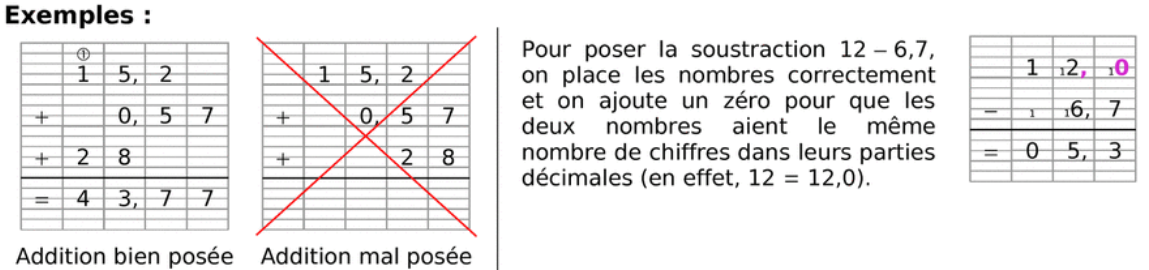
\includegraphics[scale=0.4]{img/01-addition.png}

\textbf{Attention}: Dans une somme de plusieurs termes, on peut échanger l'ordre des termes afin de simplifier le calcul. Cette opération est interdite dans une différence.

\subsection{Multiplication de nombres}
\subsubsection{Vocabulaire}
\begin{definition}{Définition}
Les nombres que l'on multiplie s'appellent les facteurs.\\
Le résultat d'une multiplication s'appelle le produit.
\end{definition}
\textbf{Exemple}: $28 = 7 \times 4$. 28 est la produit; 7 et 4 sont les facteurs.
\subsubsection{Multiplication par 10, 100, 100, ...}
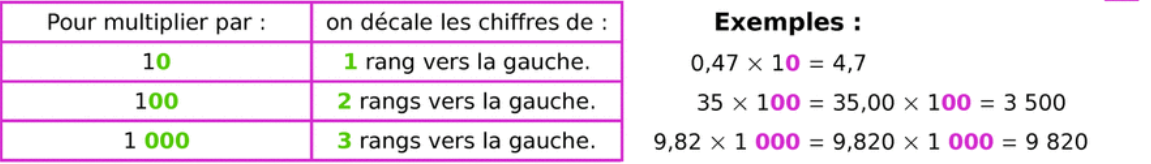
\includegraphics[scale=0.4]{img/02-multiplication.png} 
\subsubsection{Technique opératoire}
\begin{definition}{Règle}
Pour effectuer la multiplication de deux nombres décimaux,
\begin{itemize}
\item on effectue d'abord la multiplication sans tenir compte des virgules;
\item on place la virgule dans le produit en utilisant la méthode décrite ci-dessous.
\end{itemize}
\end{definition}
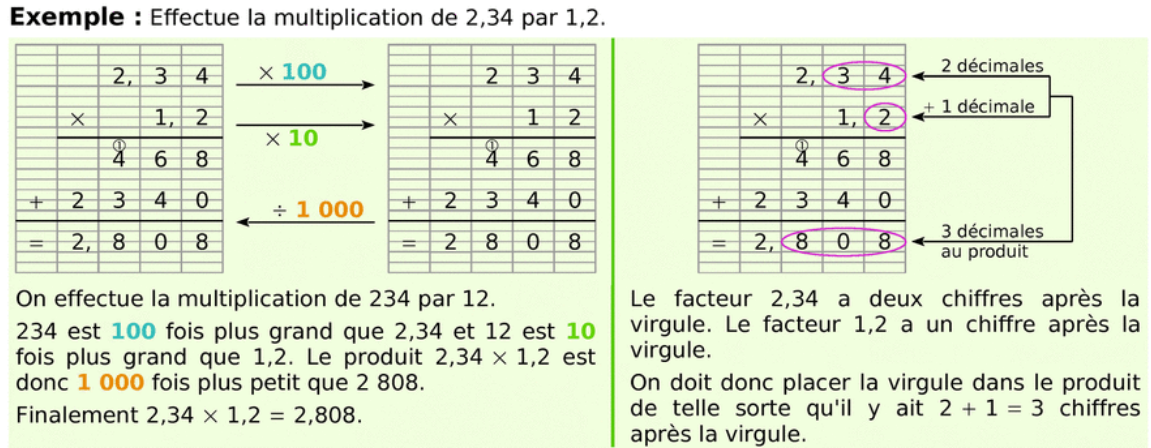
\includegraphics[scale=0.4]{img/03-multiplication.png} 

\subsection{Ordre de grandeur}
\begin{definition}{Définition}
Un ordre de grandeur d'un nombre est une valeur approchée simple de ce nombre.
\end{definition}

\textbf{Remarque}: L'ordre de grandeur d'un nombre n'est pas unique. 273,81 peut avoir comme ordre de grandeur 273, 270 voire 300. Le choix de l'ordre de grandeur dépend de la situation.

\textbf{Remarque}: Calculer avec des ordre de grandeurs permet de vérifier la cohérence d'un résultat.
\ifdefined\isprof
	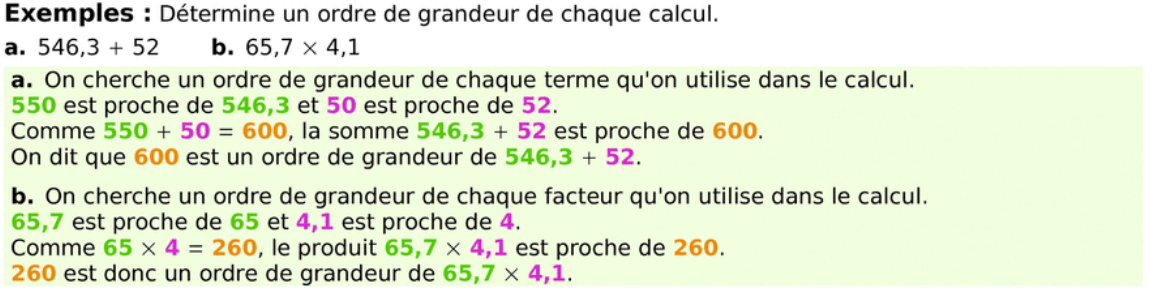
\includegraphics[scale=0.45]{img/04-ODG.png}  
\else
	\vspace{8cm}
\fi

\section{Calculer avec des durées}
\subsection{Exemple 1}
\ifdefined\isprof
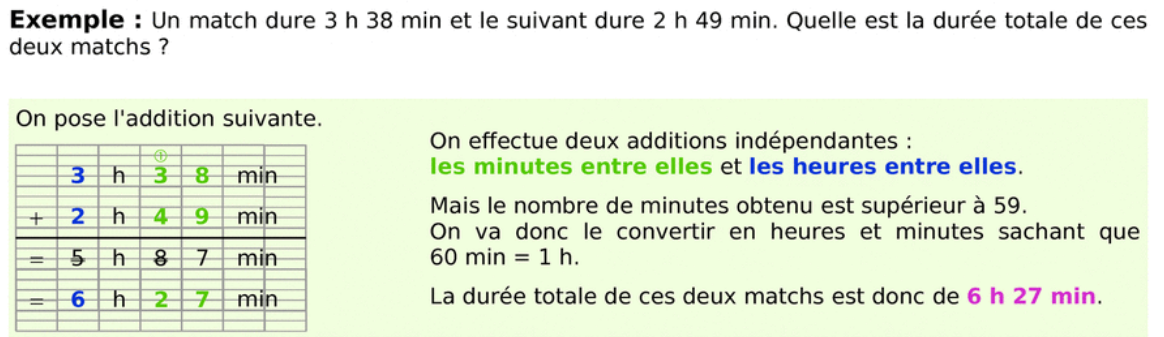
\includegraphics[scale=0.45]{img/05-addduree.png} 
\else
	\vspace{8cm}
\fi
\subsection{Exemple 2}
\ifdefined\isprof
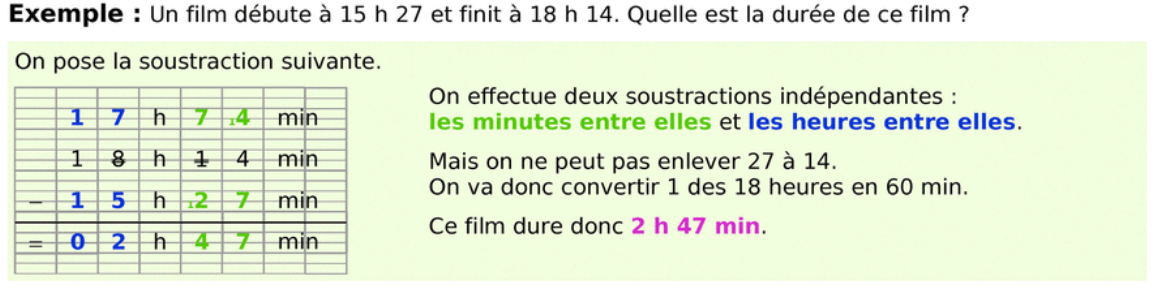
\includegraphics[scale=0.45]{img/06-subduree.png} 
\else
	\vspace{8cm}
\fi

\end{document}